%! Author = Saeid Yazdani
%! Date = 1/3/2024


\section{Design for Test}
\label{subsec:dfx-dft}

\autoref{fig:12umXray} shows a delicate x-ray image of an \ac{IC}: A direct
result of a reduction in feature size is an increased possibility of fabrication
faults within the silicon area that affect transistors and interconnects
(wires, vias, and etc.) \autocite{Laung-Terng}.

\begin{figure}[h]
    \centering
    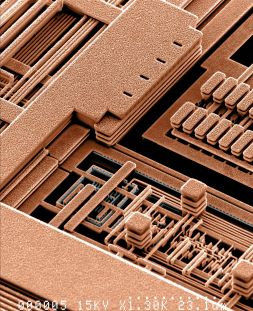
\includegraphics[scale=0.90]
    {figures/IBM_CMOS_7S_resized}
    \caption[IBM 7S Fabrication Process]
    {IBM CMOS \ac{IC} built on six layers and a transistor channel length
    of \SI{12}{\micro\meter} \autocite{645975}.
    At these dimensions, any geometrical abnormality due to the fabrication process
    or slightest exposure to dust particles can immediately cause defects in the
    product.
    The job of testing is to find this defect before shipping out the product.}
    \label{fig:12umXray}
\end{figure}

The roots of \ac{DfT} date back to the advent of digital circuits, since
there was already a proven technology from \emph{IBM}: This company had felt the
challenges with testing complex \ac{IC}s already in the 1960s, as they were
at the time, the forerunners of technology with their line of supercomputers.

\subsection{Scan Design and Scan Chains}
\label{subsec:scan-design}

In the 1970s, as the complexity of \acp{IC} began to increase, the need
for systematic testing approaches started.
Naturally, with the increase in transistor count, the number of potential faults
increased exponentially, and manual test pattern generation became inefficient,
if not impossible.

Because we cannot generate test patterns with a high fault coverage if there
are millions of gates buried behind a few interface pins or balls \acs{IBM}
invented the \ac{BILBO} \autocite{5389890} and \ac{LSSD}, that could
fulfill test requirements even under such conditions.
This led to the early introduction of \emph{Scan Design} and was
adopted by all other major companies by the 1990s \autocite{4030925}.

Through scan-based testing, all (full scan) or a selected number
of flip-flops (partial scan) will be
augmented with extra logic as shown in \autoref{fig:scan-flop-example}.
These \acp{SFF} could be connected in series to form \emph{Scan Chains} or
\emph{Scan Paths} and enter serial shift mode during the test.
\autoref{fig:scan-test-example} illustrates a logic sub-circuit with \acp{SFF}.

\begin{figure}[htbp]
    % Note: With Inkscape using electrical symbols, I scaled the logic symbols
    % to 125% as they are relatively smaller than the rest of the symbols
    \centering
    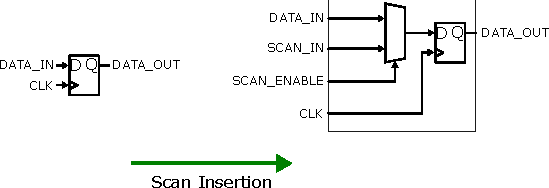
\includegraphics[width=\linewidth,height=0.62\textheight,keepaspectratio]
    {figures/normal_vs_scan_flipflop}
    \caption[Comparison of a normal and scan enabled flip-flop]{A normal
    \ac{FF} (left) and a \ac{SFF} (right). \ac{EDA} tools can help during the
    design time to convert normal \ac{FF}s to \ac{SFF} and optimally place them
    in the final synthesis. Scan enabled \ac{FF}s can help with the detection of faults
    at wafer-level and functional tests.}
    \label{fig:scan-flop-example}
\end{figure}

\begin{figure}[h!]
    \centering
    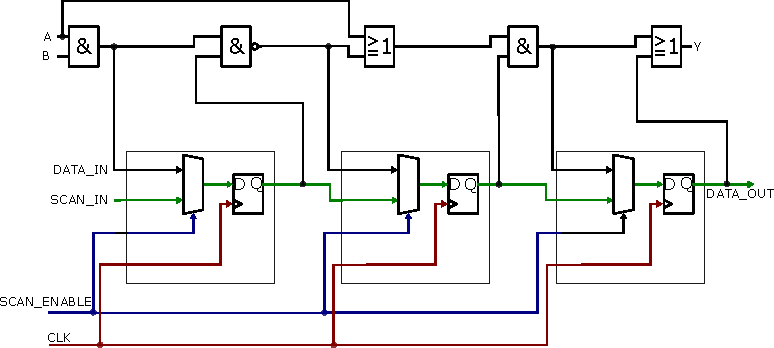
\includegraphics[width=\linewidth,height=0.62\textheight,keepaspectratio]
    {figures/scan_chain_example}
    \caption[Scan Chain Example]{An example of standard integration of
    scan-enabled \ac{FF}s in a scan-chain.
    }
    \label{fig:scan-test-example}
\end{figure}

It should be noted that the addition of \ac{SFF}s to a design will cause an
extra overhead in terms of gate count and minor timing issues, as well as
allowing malicious attacks through scan chains, especially on
encryption-related logic gates \autocite{8746214}.

\subsection{Scan Chains Drawback on \acs{ATE}-\acs{DUT} Power Supplies}
\label{subsec:scan-design-challenges-ATE-PSU}

There is one major drawback of all the serial SCAN operations: Shifting data
through the whole chip increases the total inrush current to such a level that
internal power wiring weaknesses will not stay undetected.

At each and every clock edge we transfer a charge packet between power rails for
all changing nodes, and if there is any bottleneck in the supply rail design we
get a fatal ground bounce or power line drops – both killing the normal
functionality and terminating the test process – we are not able to shift
in and out all scan data.
One major task for modern ATE DUT power supplies,
therefore, is the delivery of absolutely stable supply and ground rails at the
the DUT pins.
In consequence, we always must read the voltage rails at the DUT pins and correct
the power supply output.

Because modern logic chips are based on SCAN and \ac{BIST} testing we need
sophisticated DUT supply strategies to keep up with the demanding requirements.

As long as the DUT ATE power supplies are located in the ATE mainframe we must
rely on REMOTE sense with at least half a meter of wiring length.
The remote sense signals travel along these sense lines and reach the
mainframe long after any incident at the DUT position.
This delay is the key issue for the control loop design, and we will show
solutions in this work.

The only solution to reduce the wiring length of a remote sense line is to
bring the supply closer to the DUT.
Because we do not appreciate large power supply modules on a load board we will
use this approach only in worst cases when we need fast switching AND high
currents at the same time.
Dedicated smart power ICs are amongst such applications (PWM motor drivers,
PWM energy conversion modules, etc.)

%%%%%%%%%%%%%%%%%%%%%%%%%%%%%%%%%%%%%%%%%%%%%%%%%%%%%%%%%%%%%%%%%%%%%%%%%%%%%%%%

\subsection{Built-In Self-Test}
\label{subsec:bist}

Another approach to reducing test time at still high fault coverage was the
introduction of built-in self-test \ac{BIST}.
We can reduce the scan path lengths to a larger degree if major partitions of
the logic have their own logic \ac{BIST} controller where we only need to read
the pass/fail result from internal registers via scan.
The same is true for memory testing where \ac{MBIST} controllers reduce the
external access to some control operations.

\ac{BIST} is a structural \ac{DfT} method within an \ac{IC}, especially used in
safety-critical systems (as discussed in
\autoref{sec:history-errors-failures-in-electronic-systems}).
\ac{BIST} cores operate in one of the two following
modes: \emph{offline} or \emph{online} \autocite{953276}:

\begin{itemize}[topsep=8pt,itemsep=4pt,partopsep=4pt, parsep=4pt]
    \item \textbf{\emph{Online \ac{BIST}}:}
    Is used to continuously test logic or memory circuits
    in real-time when the device is powered up
    to either raise an interrupt to a supervisor when faults are detected,
    or, if available, re-queue the failed operation in another area
    of the chip.
    Online \ac{BIST} is either implemented \emph{concurrently}, i.e. runs
    during the
    normal operation of the device, or \emph{non-concurrent}, during idle times
    of the device by executing diagnostic macros.

    \item \textbf{\emph{Offline \ac{BIST}}:} Targets fault detection
    at the times when the device is not in its normal function mode (suspended,
    in sleep mode, etc.) and is aimed to find faults that were not found during
    online operation. Offline \ac{BIST} is used for functional and structural
    testing and does not detect run-time errors.
\end{itemize}

\ac{MBIST} is widely used for the detection of faults
in memory cells.
An \ac{IC} augmented with \ac{MBIST} will show the following reactions
of memory corruption:

\begin{itemize}[topsep=8pt,itemsep=4pt,partopsep=4pt, parsep=4pt]
    \item Mark faulty memory regions,
    \item Assert a warning signal if data corruption is detected.
\end{itemize}

\autoref{fig:memory-bist-diagram} shows a block diagram of offline
\ac{MBIST} where the built-in test controller manages various units such as
\ac{BGPG}, \ac{AG}, and multiplexers to carry offline tests on
the memory \autocite{953276}.

\begin{figure}[h!]
    \centering
    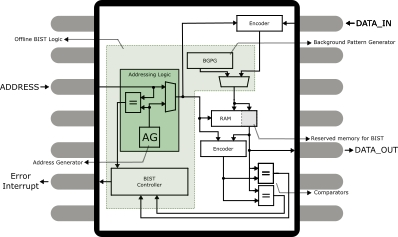
\includegraphics[width=0.80\linewidth,height=0.46\textheight,keepaspectratio]
    {figures/diagram-offline-memor-bist.jpg}
    \caption[Memory BIST Structure]{A Simplified internal block diagram of
    an \ac{MBIST} implementation.}
    \label{fig:memory-bist-diagram}
\end{figure}

When compared to scan-based testing, there are a number of noteworthy
advantages and disadvantages associated with \ac{BIST}:

\begin{itemize}[topsep=8pt,itemsep=4pt,partopsep=4pt, parsep=4pt]

    \itemcon \ac{BIST} adds complexity to design and integration.

    \itemcon \ac{BIST}  causes more silicon overhead compared to
    scan chains test structures.

    \itempro \ac{BIST} is a smart, test mechanism built into the
    device itself, while scan-based testing requires the presence of external
    \ac{ATE} for applying test patterns.

    \itempro With \ac{BIST}, test costs are reduced as an external
    \ac{ATE} is only required to power up the \acs{DUT}
    and to test areas of the chip that are not augmented with
    \ac{BIST}.

    \itempro Employing online and offline \ac{BIST}, the product can be
    monitored for health and fitness during its entire lifetime.

    \itempro \ac{BIST} uses internal dynamic pattern generators or
    pre-stored test pattern, while for scan testing, the test vectors
    come from an external \ac{ATPG}.

    \itempro \ac{BIST} tests are performed at native speeds of the \ac{DUT}
    while scan tests are dependent on the throughput of external \ac{ATE}
    hardware.

\end{itemize}

\emph{\ac{BICS}} is another variant of built-in tests and a complement of logic testing
and focuses on current monitoring in \ac{CMOS} technology, which is vital in
finding physical defects such as open-circuits, gate shorts, punch-through,
and bridging that can happen during fabrication.

\ac{BICS} performs the well-known \emph{IDDQ} measurement for quiescent mode
currents (at non-switching times) which in former days was a task
for external \ac{ATE} hardware \autocite{Nicolaidis} whereas \ac{BICS} can
carry out IDDQ tests online or offline, during the lifetime of an \ac{IC}.

\emph{\ac{ABIST}} or \ac{OBIST}, another approach to built-in test structures,
is the advent of analog \ac{BIST} cores \autocite{1604093} which allow for
testing functions of mixed-signal \ac{IC} and \acp{SoC} such as \ac{ADC} and
\ac{RF} sub-circuits \autocite{4437457}.
